\documentclass{article}
\usepackage[utf8]{inputenc}
%paquetes que usa el doc

\title{Hoja de trabajo \# 1}
\author{Luis Gerardo Morales Salazar \\Carnet: 2018-1364\\ morales181364@unis.edu.gt}
\date{25 de Julio de 2018}

% datos del encabezado o titulo del doc
\usepackage{natbib}
\usepackage{graphicx}


\begin{document}
\maketitle
% bloque de respuestas del ejercicio 2
\section{Ejercicio \# 2}

% imagen de dados que venia en la hoja de trabajo
\begin{figure}[h!]
\centering
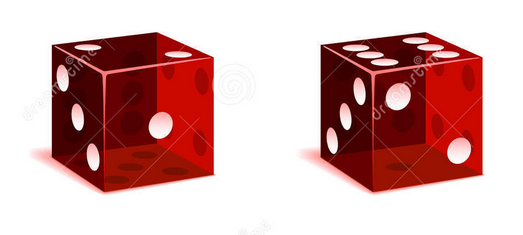
\includegraphics[scale=0.2] {die}
\end{figure}

%respuesta del grafo
\begin{enumerate}
\item Nodos del grafo: $\{1, 2, 3, 4, 5, 6\}$

\item {El conjunto de vertices del grafo son:
$\newline\lbrace<2,6>,<6,5>,<5,1>,<2,1>\rbrace
\newline\lbrace<2,3>,<3,5>,<5,4>,<4,1>\rbrace
\newline\lbrace<1,3>,<3,6>,<6,4>,<4,1>\rbrace
\newline\lbrace<1,2>,<2,6>,<2,3>,<5,1>\rbrace
\newline\lbrace<1,5>,<3,6>,<6,2>,<5,3>\rbrace
\newline\lbrace<4,1>,<4,6>,<6,3>,<4,2>\rbrace$
}

\end{enumerate}

% bloque de respuestas del ejercicio 3
\section{Ejercicio \# 3}
\begin{enumerate}
%respuesta 1 del inciso 3
\item La estructura de datos que se utiliza es la de camino.

%respuesta 2 del inciso 3
\item El algoritmo se da en la utilizar los estructura de datos de tipo camino para no limitar la posibilidad de pasar por el mismo número que ya paso anteriormente en el lanzamiento.

%respuesta 3 del inciso 3
\item Para que el algoritmo siempre produsca un resultado no tiene que tener un ciclo.
% documento creado en sharelatex.com
\end{enumerate}
\end{document}
